\documentclass{article}
\usepackage[utf8]{inputenc}
\usepackage{graphicx}
\usepackage{amsmath}
\usepackage{geometry}
\usepackage{longtable}
\usepackage{url}
\bibliographystyle{ieeetran}
\geometry{margin=1cm}

\title{\textbf{COMP90086 - Computer Vision - Assignment 1}}
\author{Jule Valendo Halim - 1425567}

\begin{document}
\pagenumbering{gobble}
\maketitle

\section*{Question 1}

My filter is implemented as a 15x15 box filter, along with a padding of 20 pixels. The result of the box filter is that the image becomes blurrier. As seen in figure \ref{fig:boxfilter1}, after filtering and zero-padding, there is a black border around the image, and the original image has become more blurred. 

Observing the log magnitude, the original image has a much brighter spots pointing towards multiple directions. There is generally less magnitude towards the higher frequency areas of the log magnitude. This could be because the image is generally bright, being filled with a lot of white. Comparing this to the filtered log magnitude, there is a more grid-like pattern. This is most likely caused by the box filter averaging the values in the image, thus each pixel is closer to the value of the pixels around it. However, it still keeps the pattern of having less magnitude for higher frequencies.

The phase of both the original and the filtered image both show complex patterns. A difference between the two is that the original image's phase has a strong vertical line, while the filtered image has both vertical and horizontal line. As the box filter averages the image values, it could cause more symmetry in the image, thus reflecting the vertical line onto the horizontal plane.

\begin{figure}[h!]
    \centering
    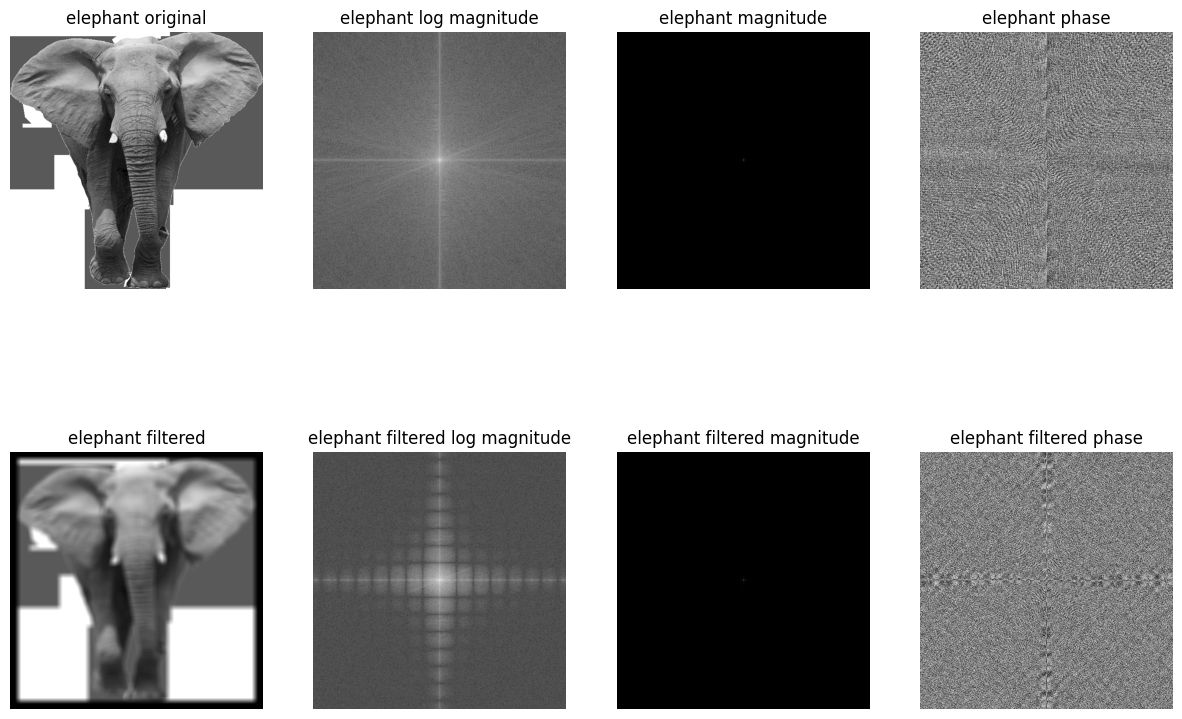
\includegraphics[scale=0.5]{images/box_filter_elephant.png}
    \caption{Collection of outputs from image box filtering}
    \label{fig:boxfilter1}
\end{figure}
\newpage
\section*{Question 2}

To calculate the object size in the image space, we first calculate the distance to object based on its given pixel coordinates. this is given as 

\[
\text{focal length in pixels} = \left(\frac{\text{focal length in mm}}{\text{sensor width in mm}}\right) \times \text{image width in pixels}
\]

\begin{figure}[h!]
    \centering
    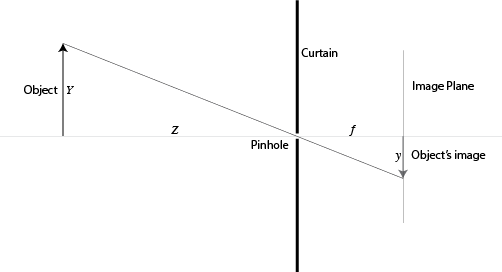
\includegraphics[scale=0.5]{images/objectsize.png}
    \caption{Image showing pinhole camera principles \cite{imageformation}}
    \label{fig:objectsize}
\end{figure}

The distance to the object in metres can then be calculated using the pinhole camera principles, which is that size of object in image / focal length of lens is equal to real world size of object /  distance from the camera to the object. Figure \ref{fig:objectsize} shows the diagram representation of this principle. This is given as: 

\[
\frac{Y}{Z} = \frac{y}{f}
\]

Where

Y = height of the object

Z = distance from pinhole

f = focal length 

y = object height in image space (using the assumption that the y in coordinate space is directly proportional to its image height)

And reformulating to find Z, we have

\[
Z = \frac{fY}{y}
\]

Using the same formula, we can reformulate to find the object height in pixel space, based on the estimated distance to the object obtained above. This is calculated as:

\[
y = \frac{fY}{Z}
\]

The object is then rescaled and the aspect ratio is maintained. The first two images in figure \ref{fig:animal_grid} shows the elephant being placed on two different areas. However, as the elephant is quite large, it is difficult to determine the change in size. The images of the dogs better highlight the difference in sizes, as dog two is placed close to the camera, the dog is larger and dog one is smaller as it is placed further away.


\begin{figure}[h!]
    \centering
    \begin{tabular}{cc}
        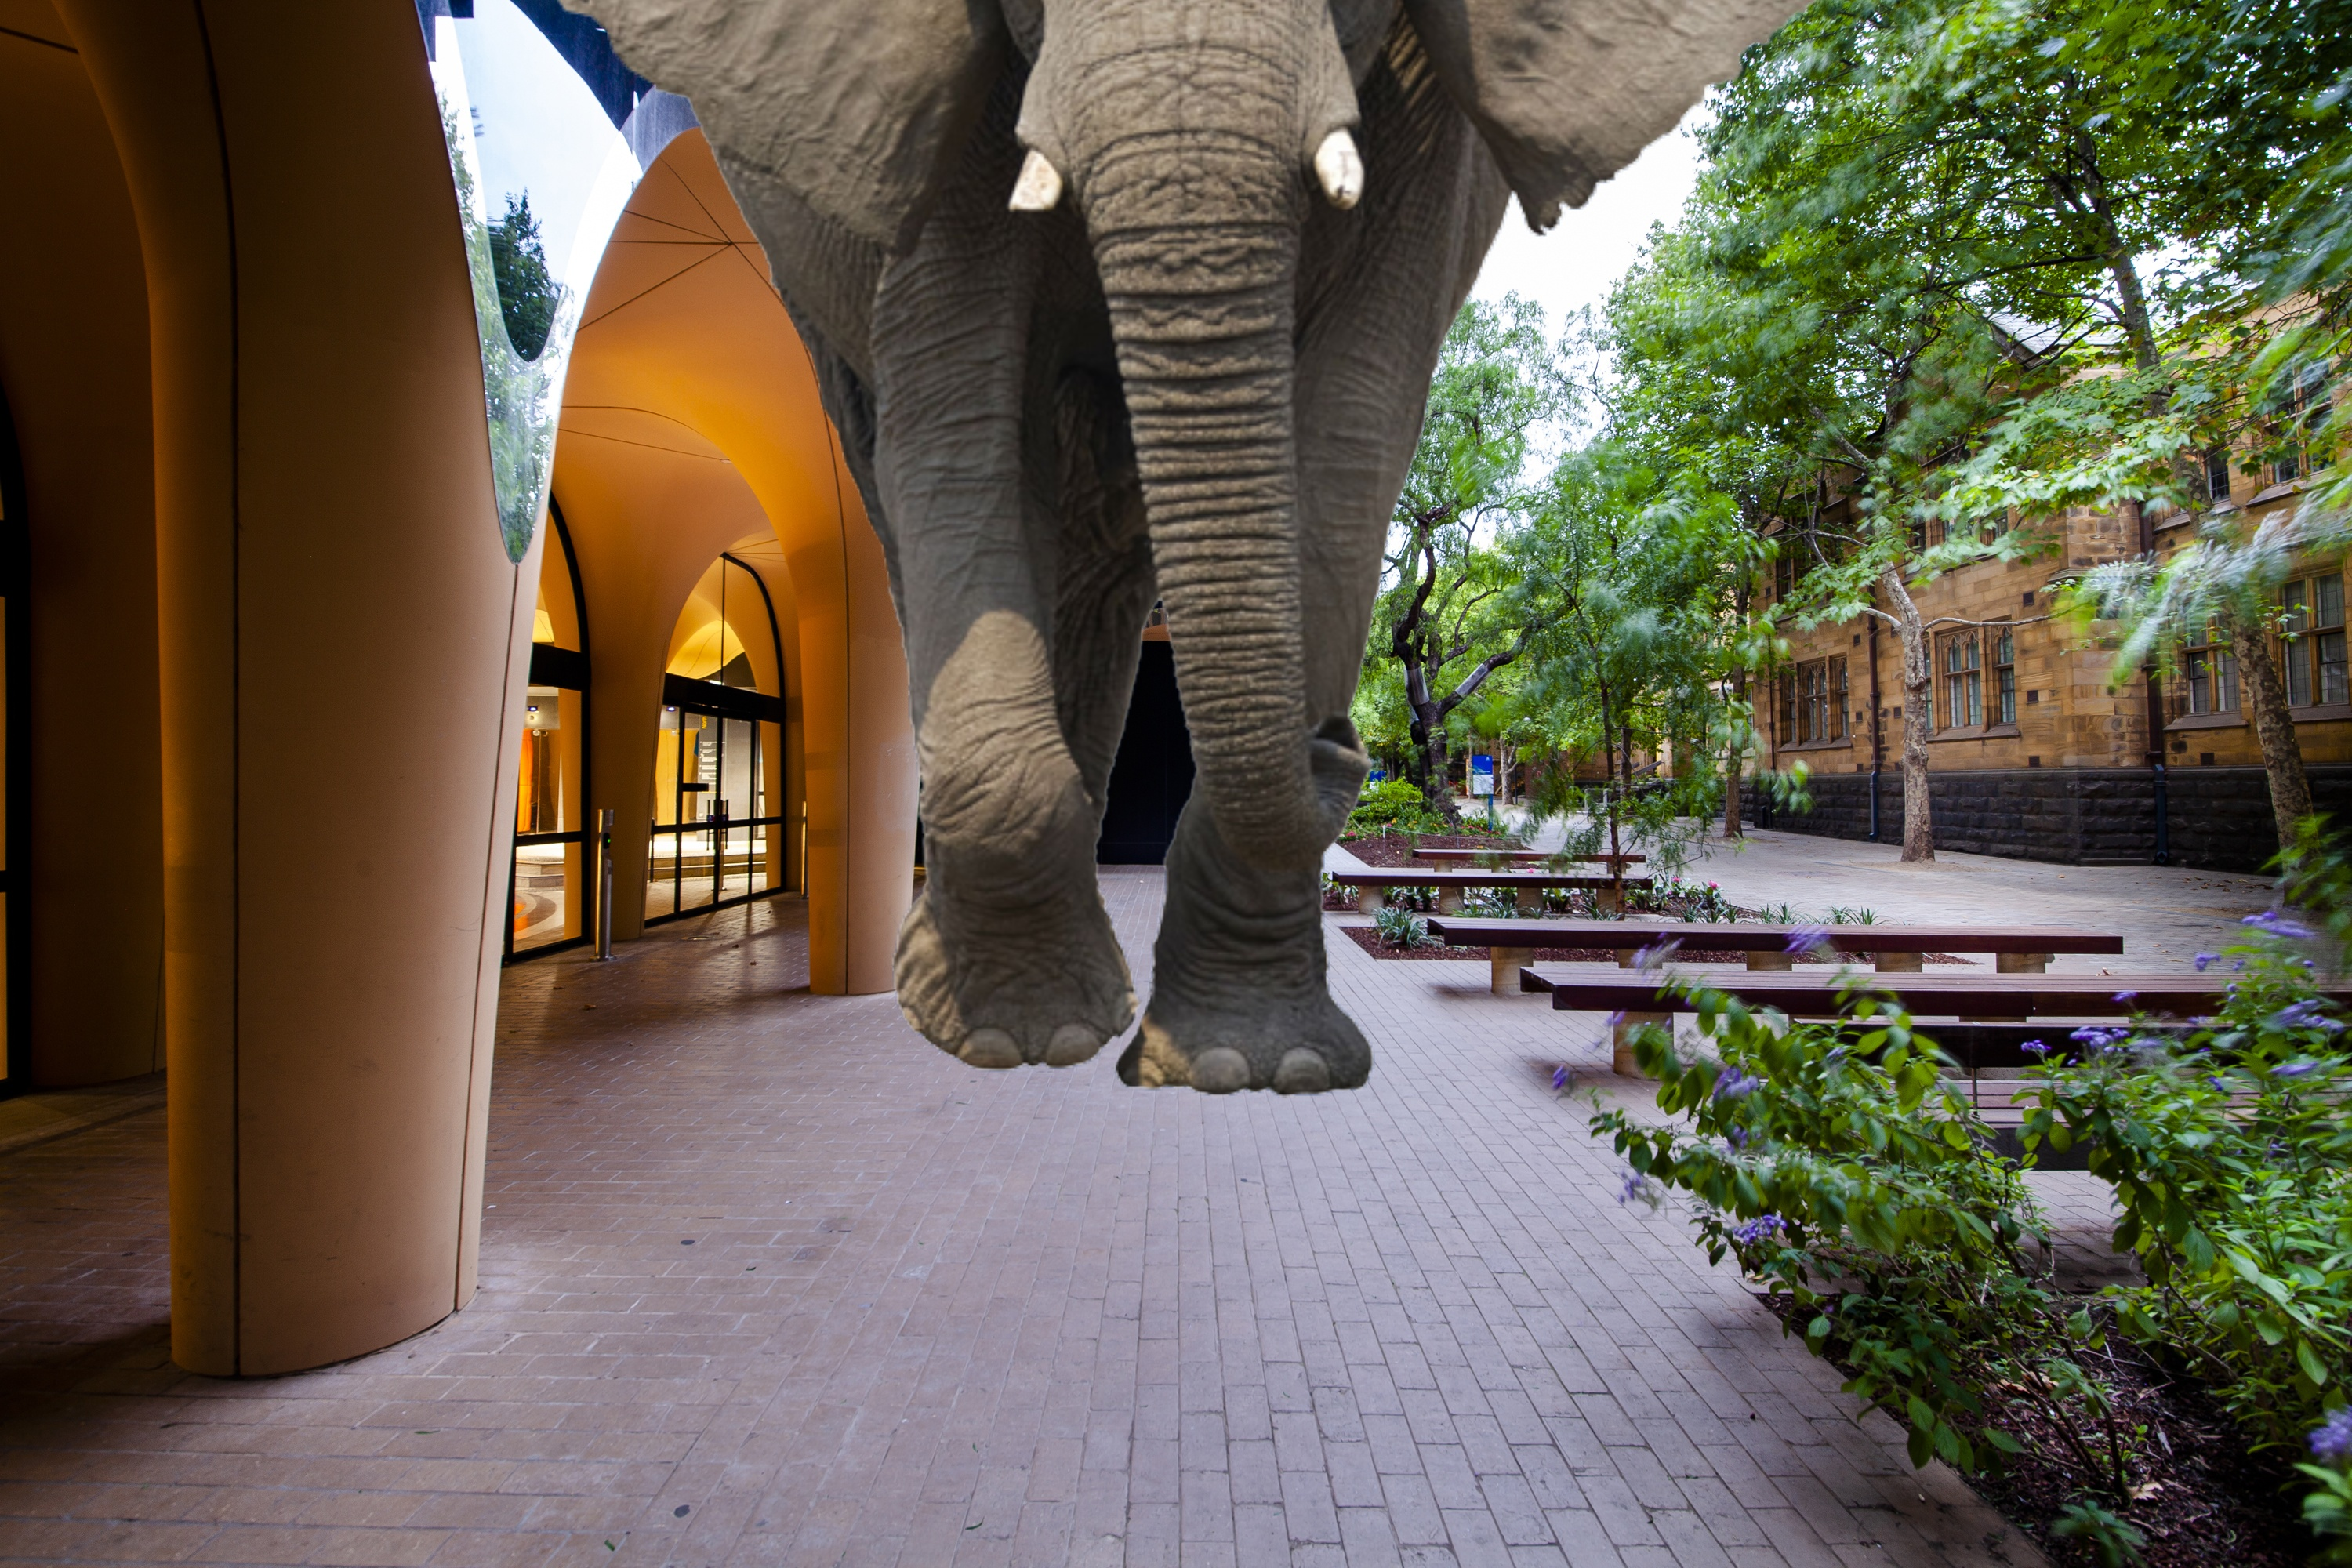
\includegraphics[scale=0.08]{images/elephant(1500x1400).jpg} & 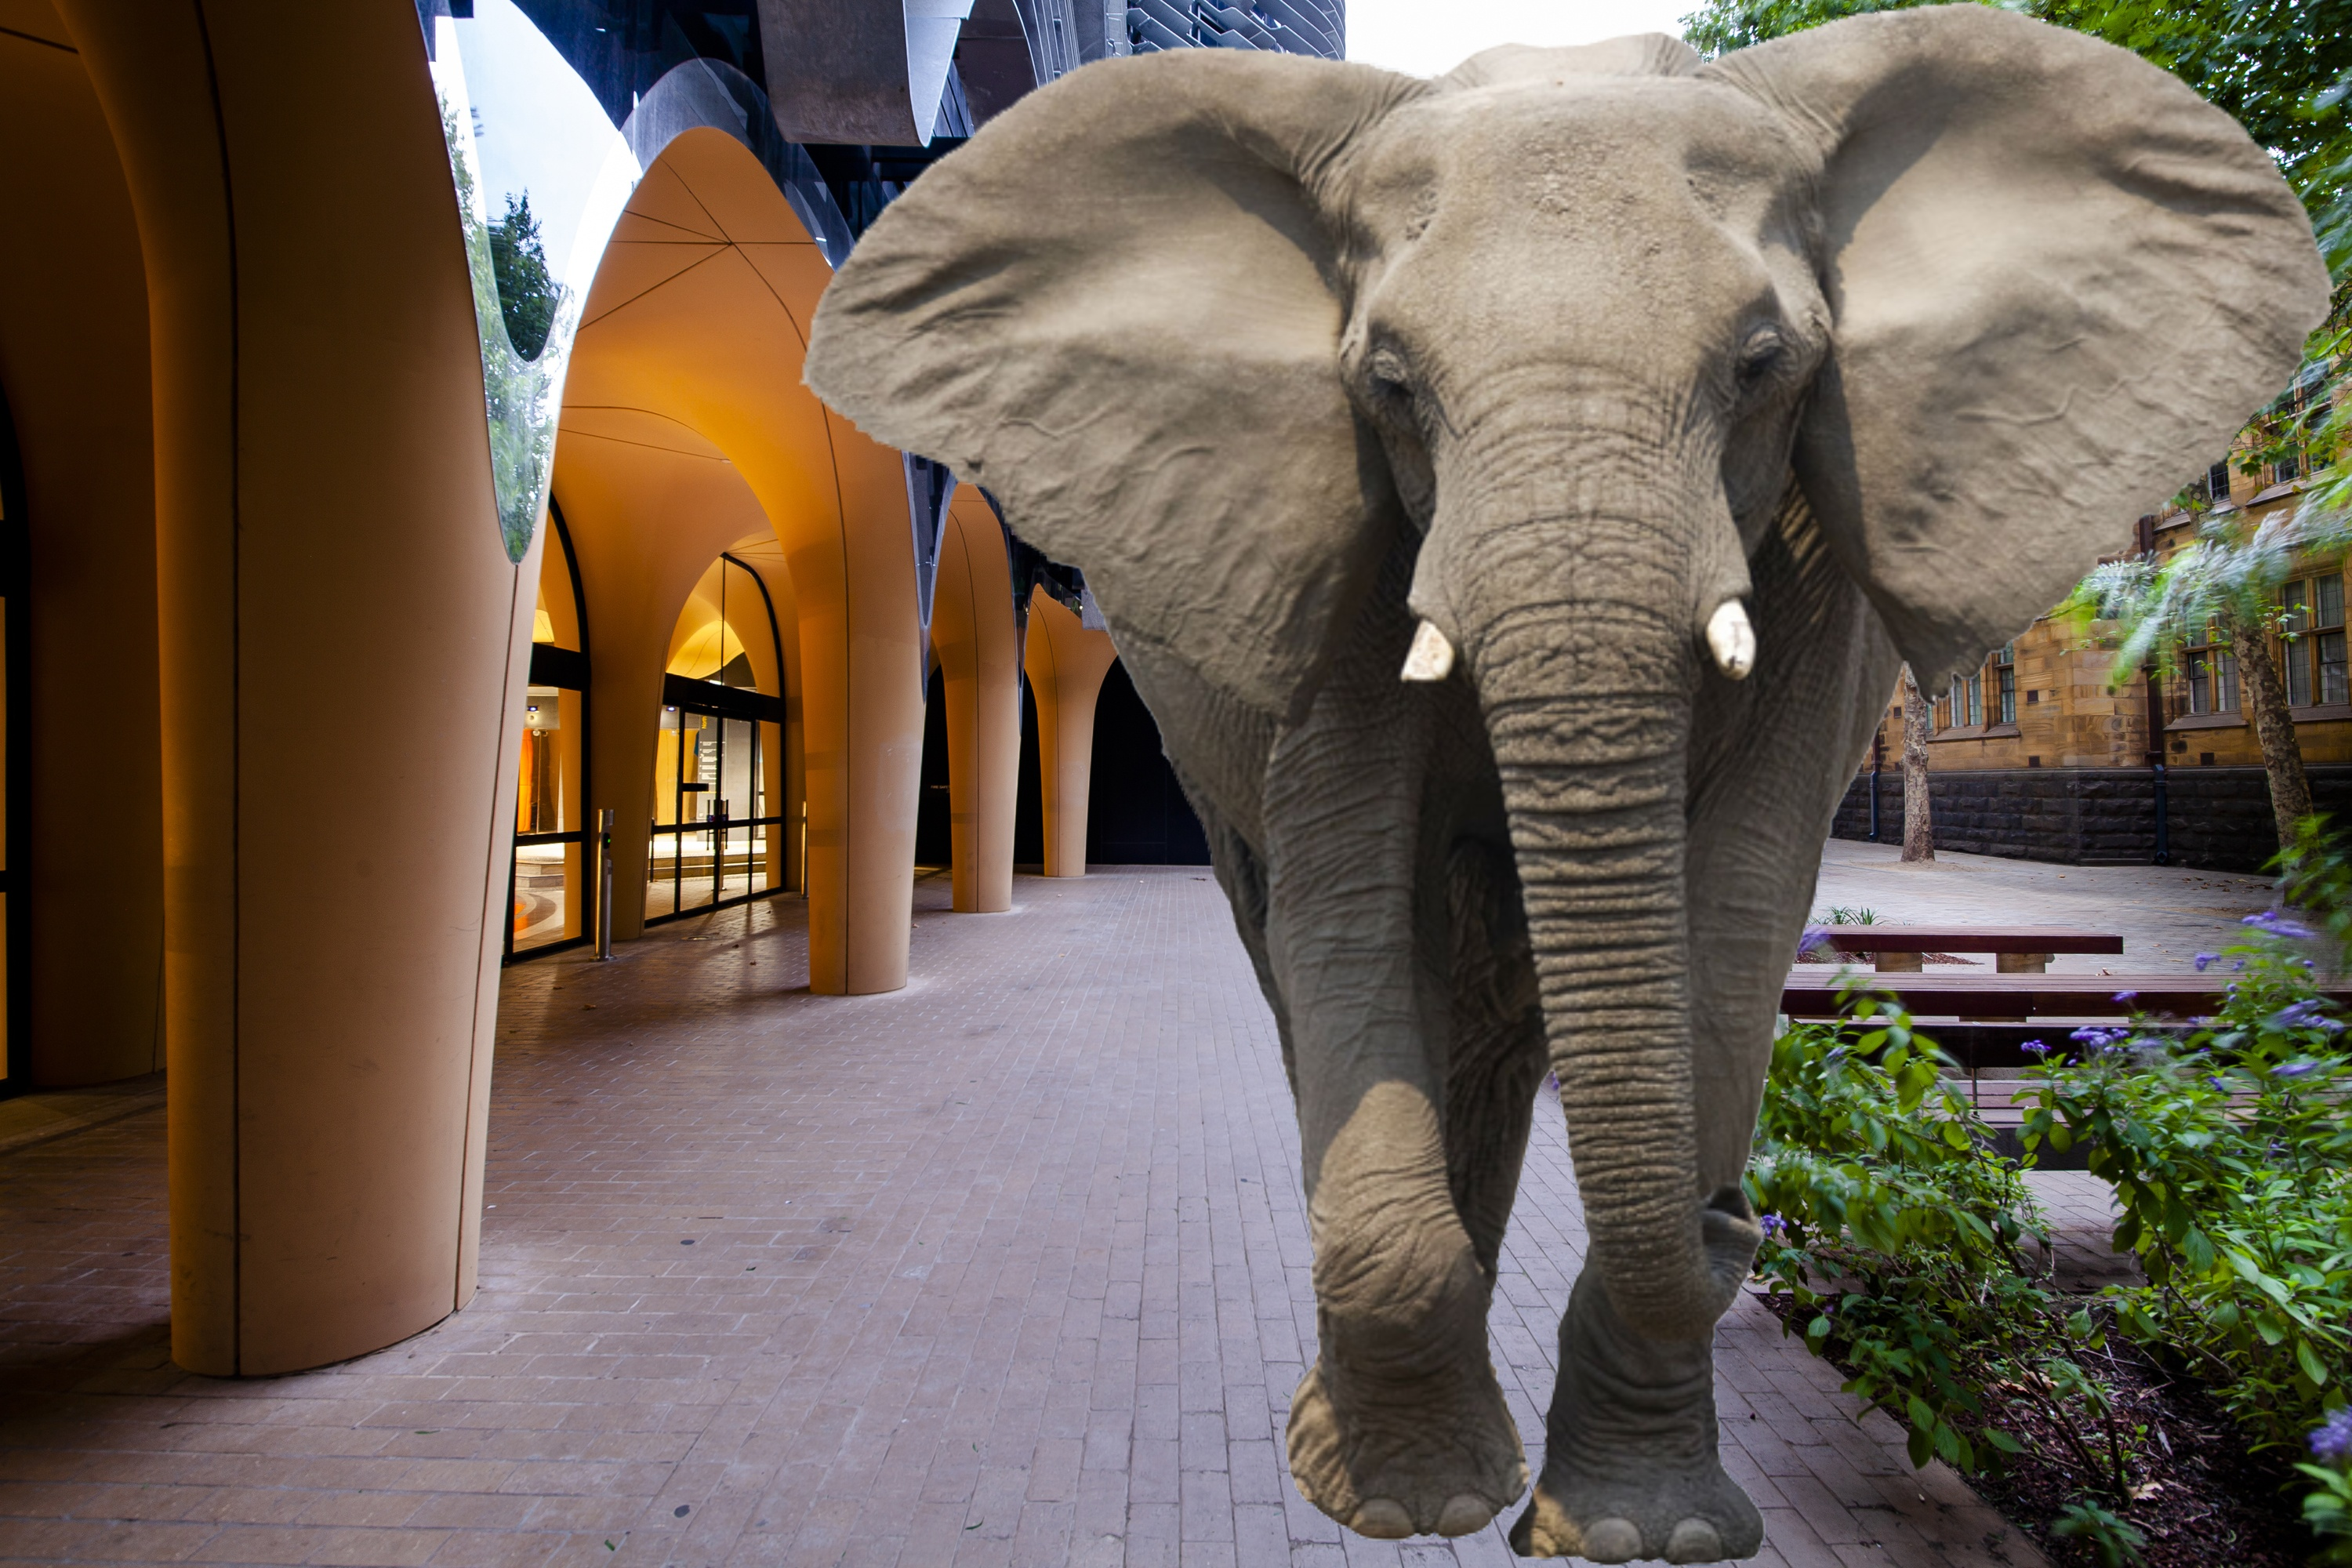
\includegraphics[scale=0.08]{images/elephant(2000x2000).jpg} \\
        Elephant One & Elephant Two \\
        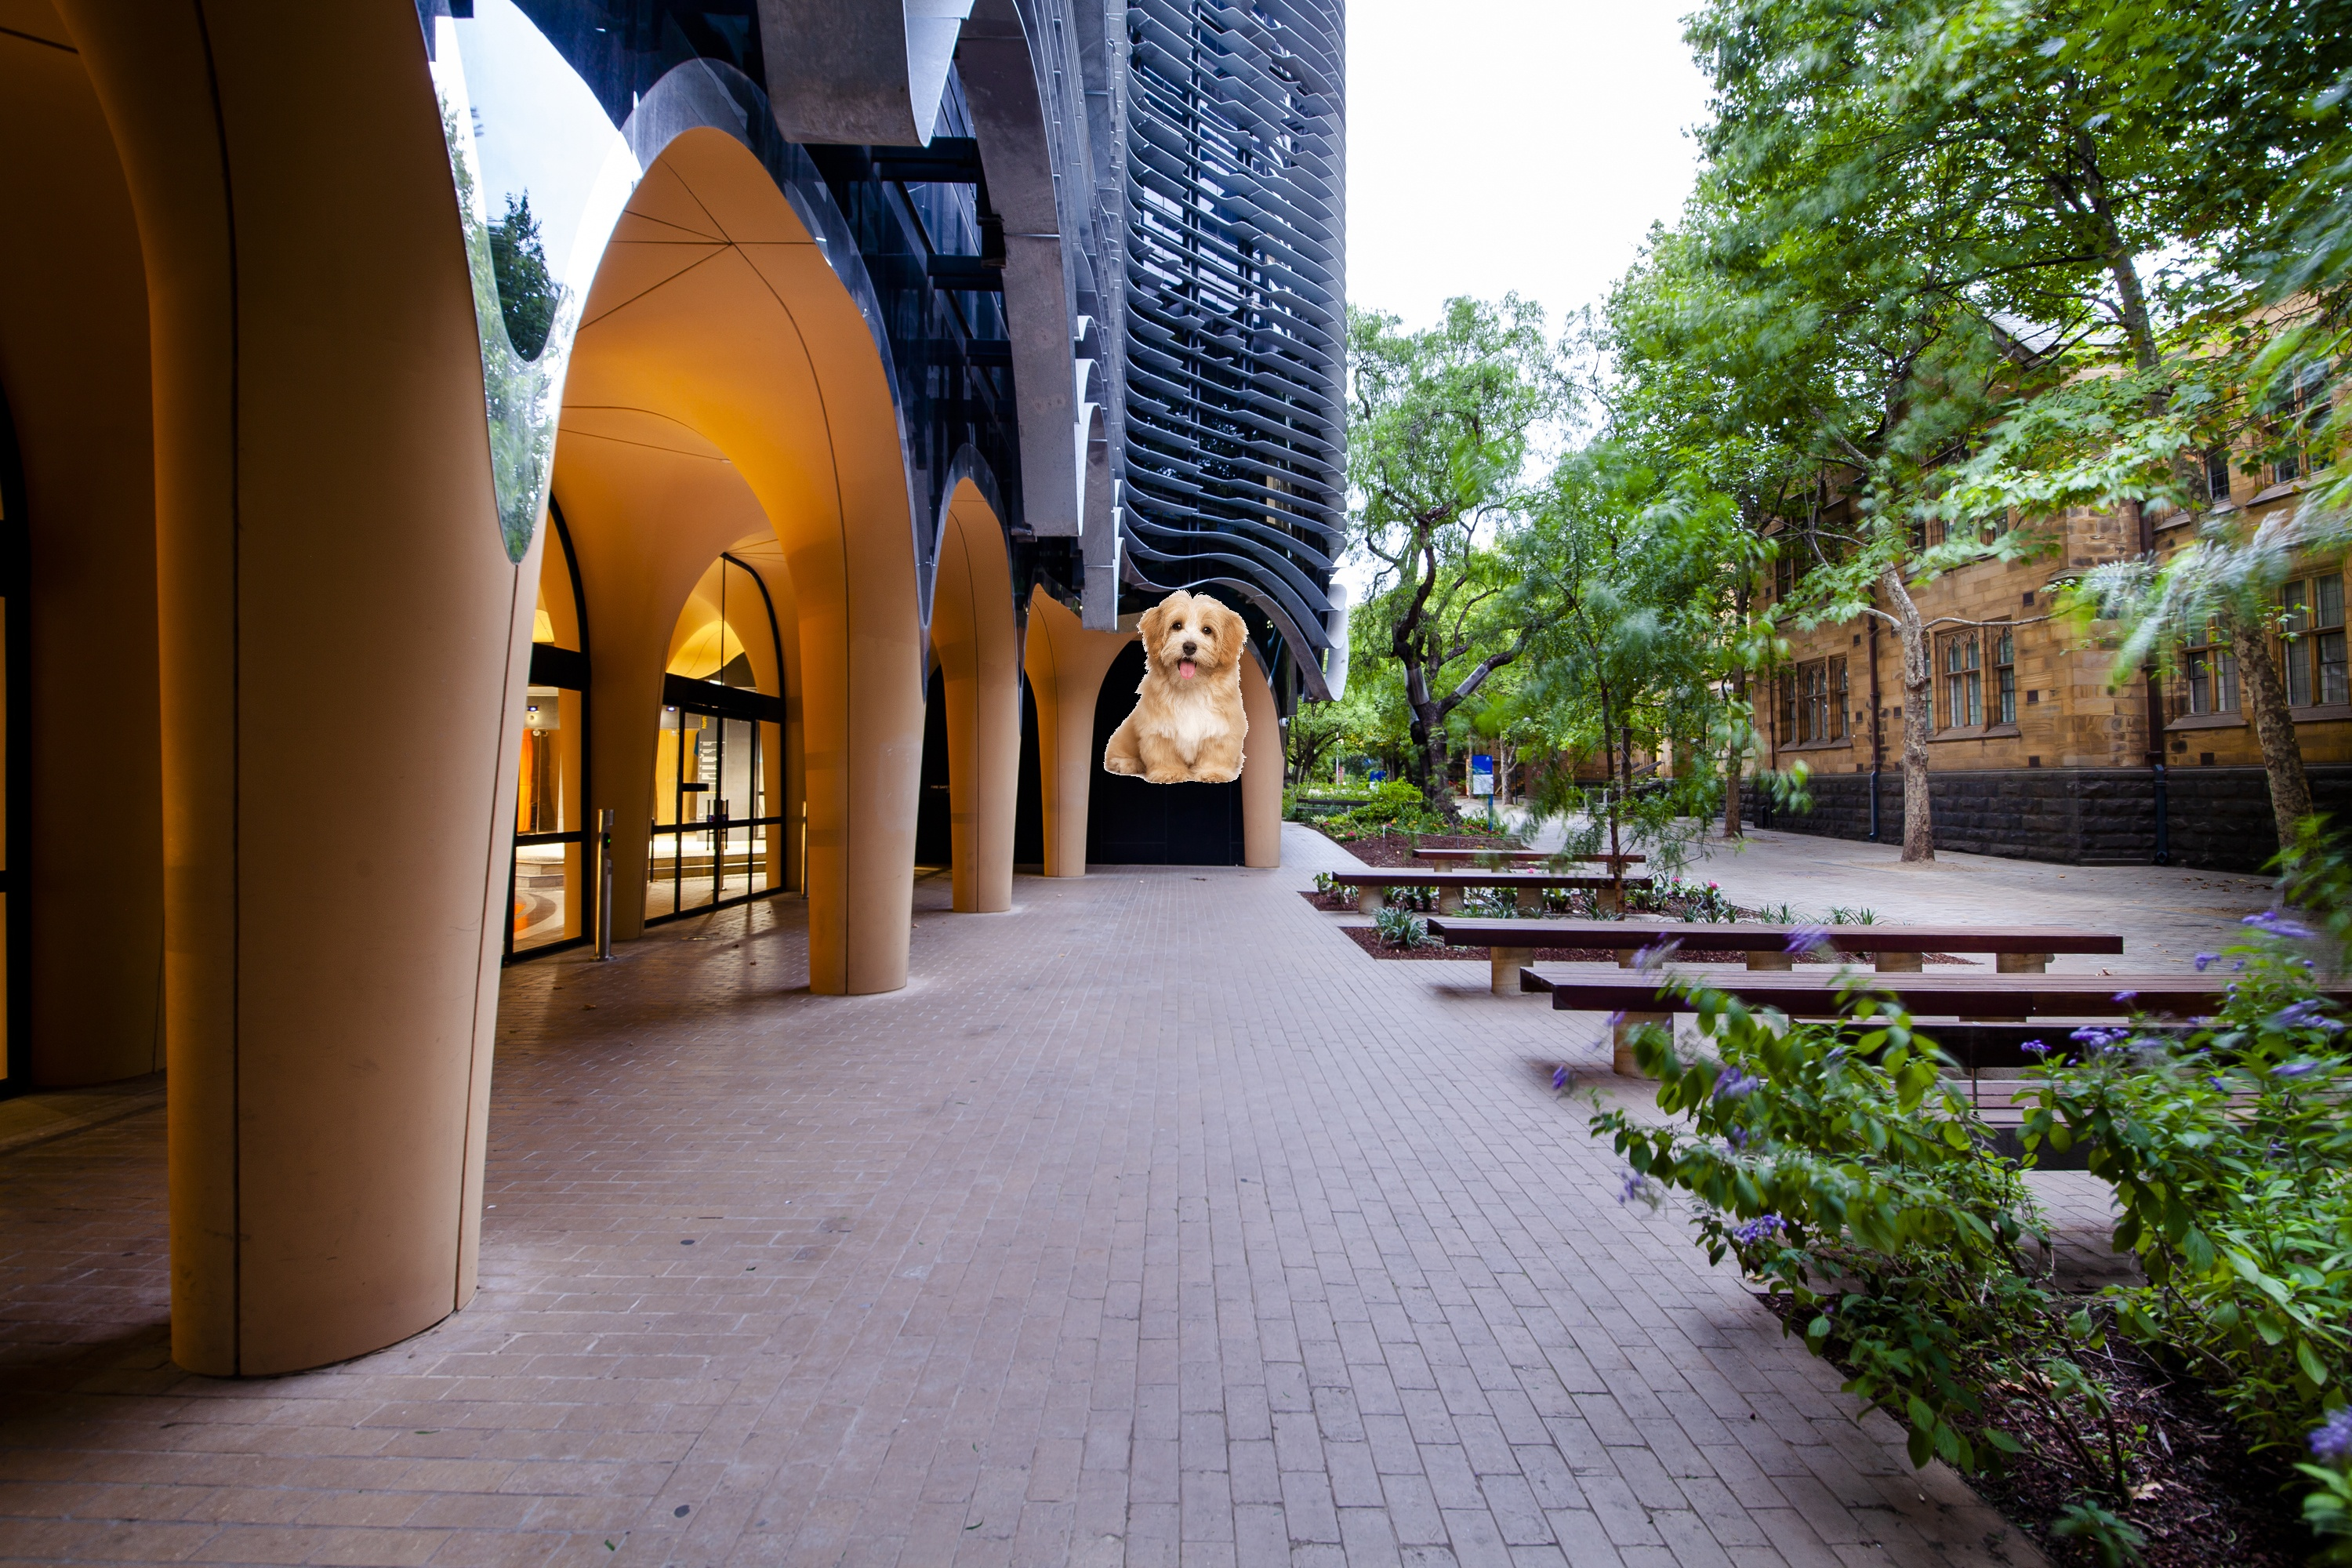
\includegraphics[scale=0.08]{images/dog(1500x1000).jpg} & 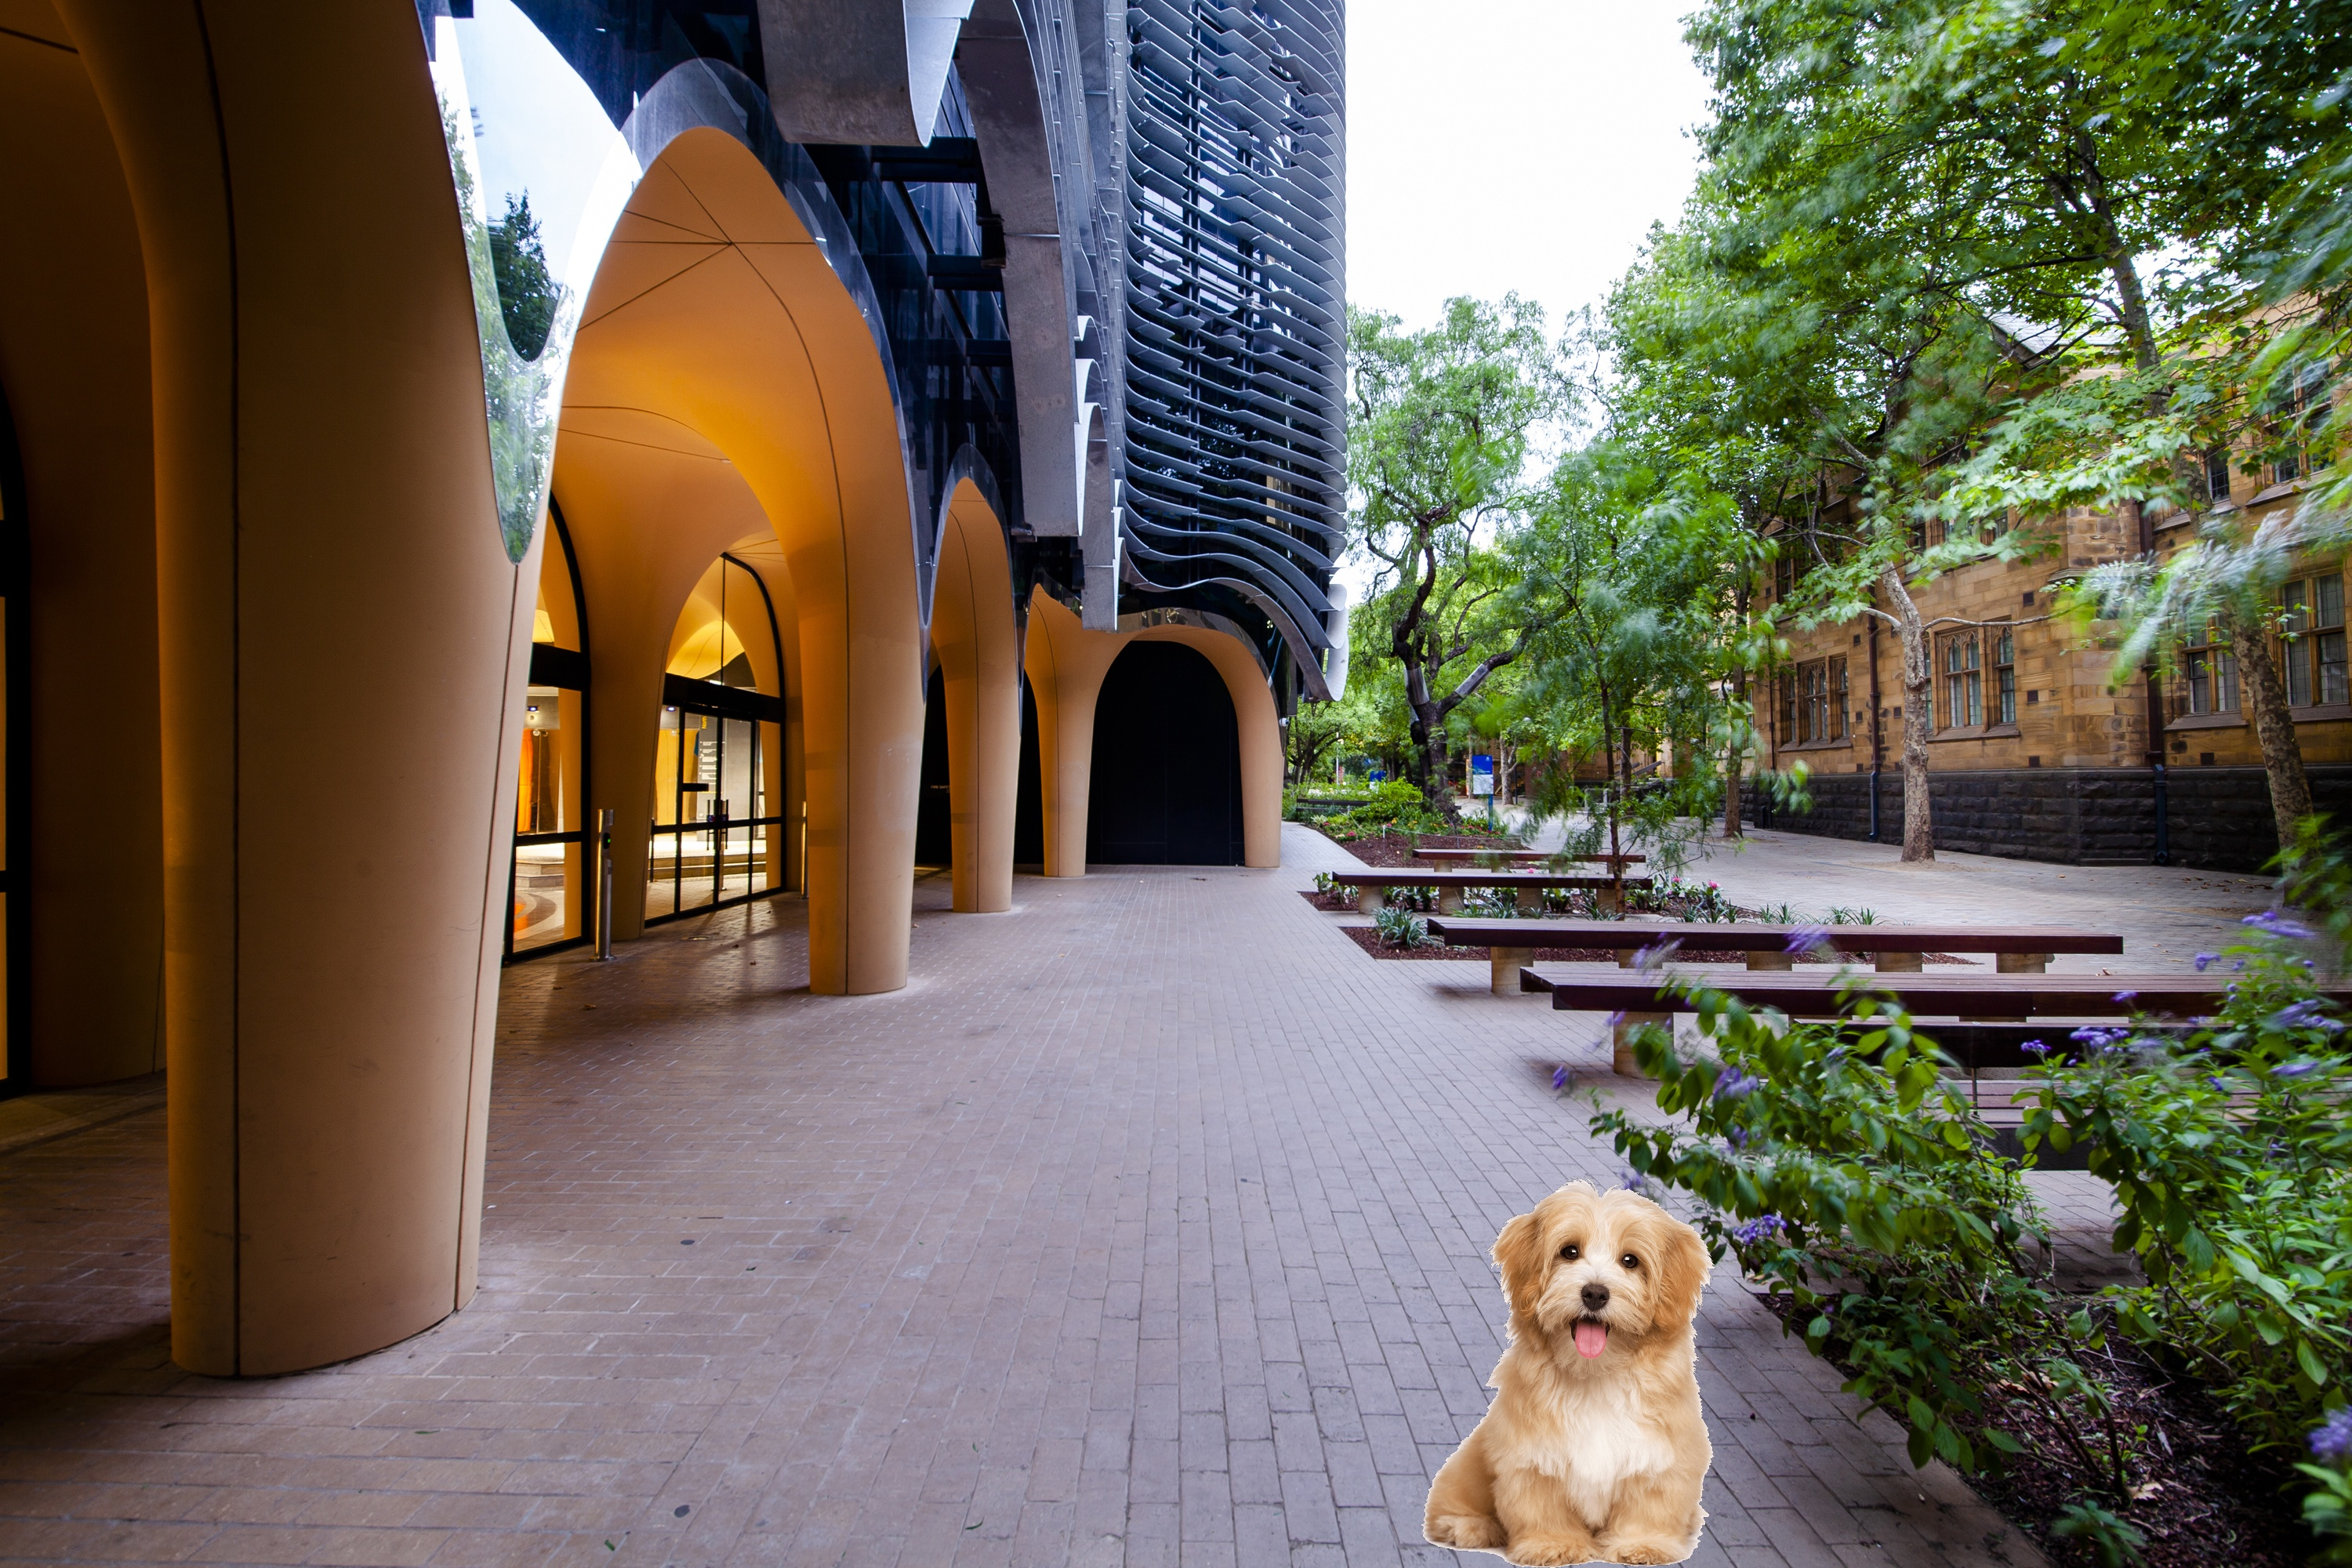
\includegraphics[scale=0.08]{images/dog(2000x2000).jpg} \\
        Dog One & Dog Two \\
    \end{tabular}
    \caption{Elephant and Dog at different positions}
    \label{fig:animal_grid}
\end{figure}

\newpage

\bibliography{custom}

\end{document}
